\documentclass[tikz,border=10pt]{standalone}
\usepackage{tikz}
\usetikzlibrary{positioning,shapes.geometric,arrows.meta,calc,fit,backgrounds,patterns}
\usepackage{xcolor}

% Define colors
\definecolor{bluelight}{RGB}{100,150,230}
\definecolor{whitelight}{RGB}{255,200,100}
\definecolor{fusioncolor}{RGB}{255,120,150}
\definecolor{headcolor}{RGB}{150,200,150}

\begin{document}

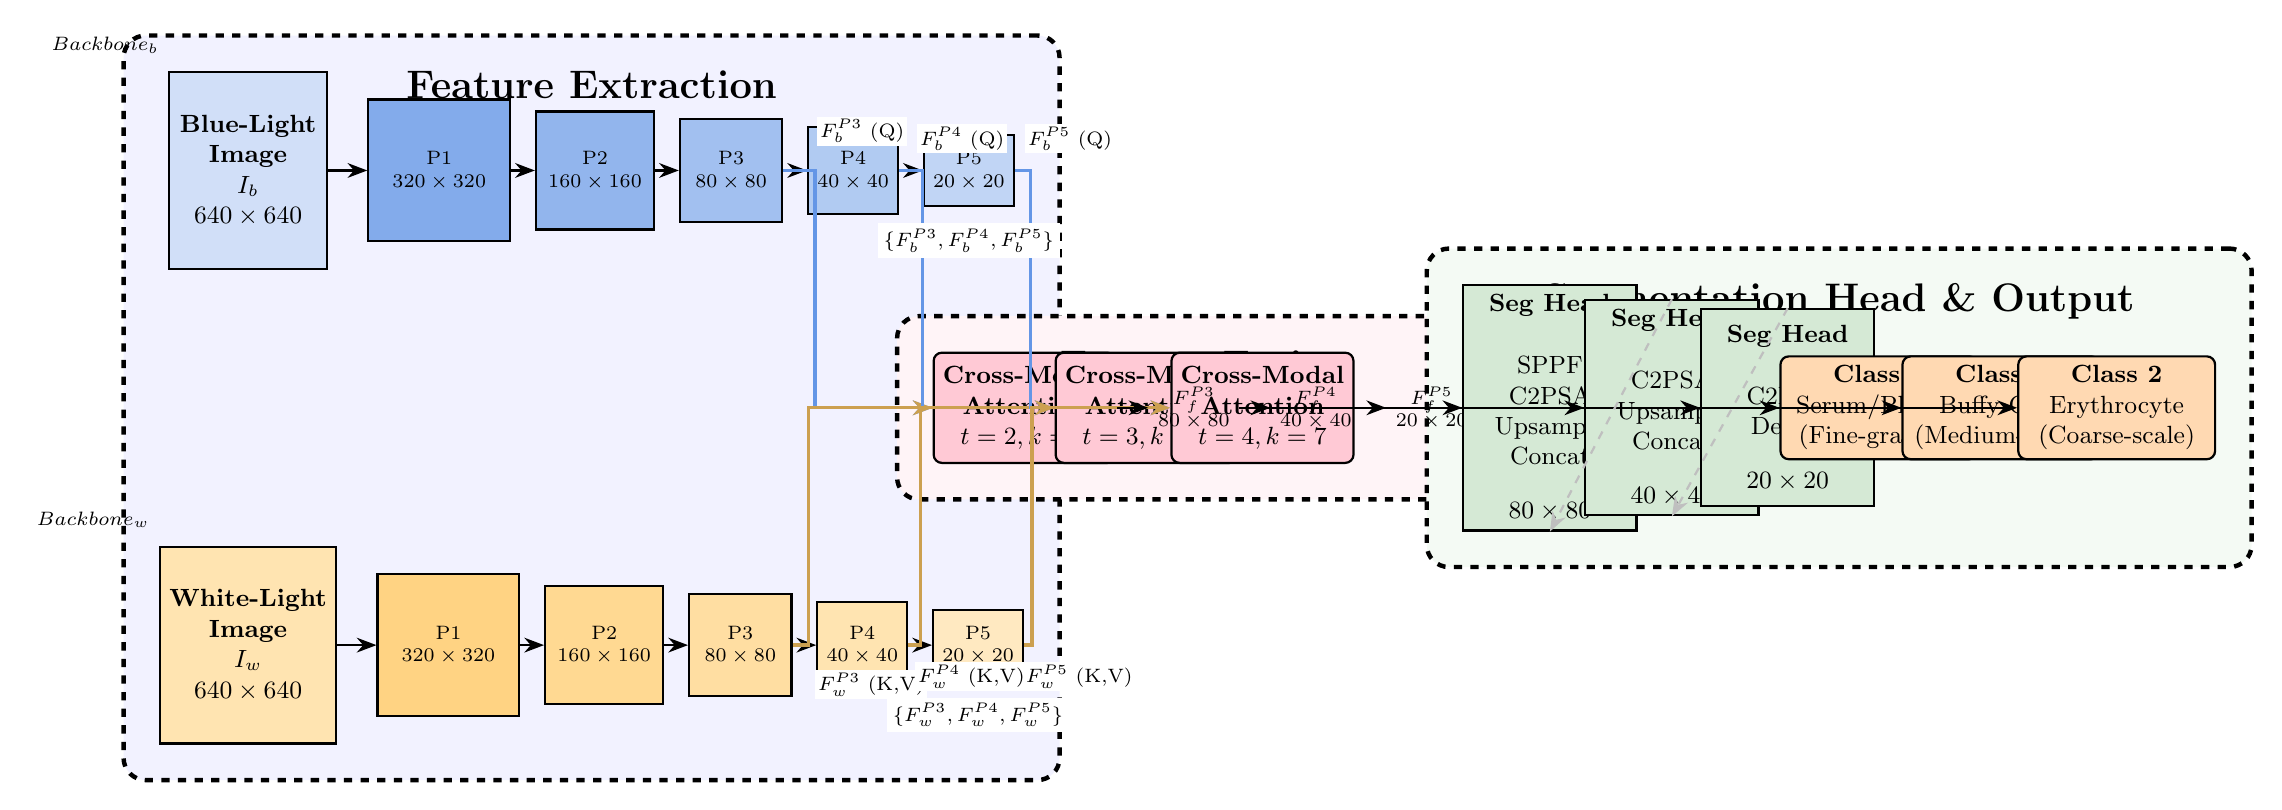
\begin{tikzpicture}[
    node distance=0.3cm and 0.3cm,
    pyramid/.style={rectangle, draw, thick, align=center, font=\scriptsize},
    fusion/.style={rectangle, draw, thick, fill=fusioncolor!40, minimum height=1.4cm, minimum width=2.2cm, align=center, font=\small\bfseries, rounded corners=3pt},
    head/.style={rectangle, draw, thick, fill=headcolor!40, minimum height=2.5cm, minimum width=2.2cm, align=center, font=\small},
    input/.style={rectangle, draw, thick, minimum height=2.5cm, minimum width=2cm, align=center, font=\small\bfseries},
    output/.style={rectangle, draw, thick, fill=orange!30, minimum height=1.1cm, minimum width=2.5cm, align=center, font=\small, rounded corners=3pt},
    arrow/.style={-{Stealth[length=2.5mm]}, thick},
    annotation/.style={font=\scriptsize, align=center},
    labelstyle/.style={font=\scriptsize\itshape}
]

%% ============ Feature Extraction - Blue Light ============
% Blue-light input
\node[input, fill=bluelight!30] (blue_input) at (0,3) {Blue-Light\\Image\\$I_b$\\$640 \times 640$};

% Blue-light pyramid layers (horizontal, aligned at center)
\node[pyramid, fill=bluelight!80, minimum width=1.8cm, minimum height=1.8cm, right=0.5cm of blue_input] (bp1) {P1\\$320 \times 320$};
\node[pyramid, fill=bluelight!70, minimum width=1.5cm, minimum height=1.5cm, right=of bp1, yshift=0cm] (bp2) {P2\\$160 \times 160$};
\node[pyramid, fill=bluelight!60, minimum width=1.3cm, minimum height=1.3cm, right=of bp2, yshift=0cm] (bp3) {P3\\$80 \times 80$};
\node[pyramid, fill=bluelight!50, minimum width=1.1cm, minimum height=1.1cm, right=of bp3, yshift=0cm] (bp4) {P4\\$40 \times 40$};
\node[pyramid, fill=bluelight!40, minimum width=0.9cm, minimum height=0.9cm, right=of bp4, yshift=0cm] (bp5) {P5\\$20 \times 20$};

% Arrows for blue pyramid
\draw[arrow] (blue_input) -- (bp1);
\draw[arrow] (bp1) -- (bp2);
\draw[arrow] (bp2) -- (bp3);
\draw[arrow] (bp3) -- (bp4);
\draw[arrow] (bp4) -- (bp5);

% Backbone label
\node[labelstyle, above left=0.1cm and 0cm of blue_input.north west] {$Backbone_b$};

%% ============ Feature Extraction - White Light ============
% White-light input
\node[input, fill=whitelight!50, below=3.5cm of blue_input] (white_input) {White-Light\\Image\\$I_w$\\$640 \times 640$};

% White-light pyramid layers (horizontal, aligned)
\node[pyramid, fill=whitelight!80, minimum width=1.8cm, minimum height=1.8cm, right=0.5cm of white_input] (wp1) {P1\\$320 \times 320$};
\node[pyramid, fill=whitelight!70, minimum width=1.5cm, minimum height=1.5cm, right=of wp1, yshift=0cm] (wp2) {P2\\$160 \times 160$};
\node[pyramid, fill=whitelight!60, minimum width=1.3cm, minimum height=1.3cm, right=of wp2, yshift=0cm] (wp3) {P3\\$80 \times 80$};
\node[pyramid, fill=whitelight!50, minimum width=1.1cm, minimum height=1.1cm, right=of wp3, yshift=0cm] (wp4) {P4\\$40 \times 40$};
\node[pyramid, fill=whitelight!40, minimum width=0.9cm, minimum height=0.9cm, right=of wp4, yshift=0cm] (wp5) {P5\\$20 \times 20$};

% Arrows for white pyramid
\draw[arrow] (white_input) -- (wp1);
\draw[arrow] (wp1) -- (wp2);
\draw[arrow] (wp2) -- (wp3);
\draw[arrow] (wp3) -- (wp4);
\draw[arrow] (wp4) -- (wp5);

% Backbone label
\node[labelstyle, above left=0.1cm and 0cm of white_input.north west] {$Backbone_w$};

%% ============ Feature Fusion ============
\coordinate (mid_point) at ($(bp3)!0.5!(wp3)$);

% Fusion modules - aligned with corresponding pyramid levels
\node[fusion, right=2.5cm of mid_point] (fusion_p3) {Cross-Modal\\Attention\\$t=2, k=3$};

\coordinate (mid_p4) at ($(bp4)!0.5!(wp4)$);
\node[fusion, right=2.5cm of mid_p4] (fusion_p4) {Cross-Modal\\Attention\\$t=3, k=5$};

\coordinate (mid_p5) at ($(bp5)!0.5!(wp5)$);
\node[fusion, right=2.5cm of mid_p5] (fusion_p5) {Cross-Modal\\Attention\\$t=4, k=7$};

% Fused feature labels
\node[annotation, right=0.4cm of fusion_p3] (fp3) {$F_f^{P3}$\\$80 \times 80$};
\node[annotation, right=0.4cm of fusion_p4] (fp4) {$F_f^{P4}$\\$40 \times 40$};
\node[annotation, right=0.4cm of fusion_p5] (fp5) {$F_f^{P5}$\\$20 \times 20$};

% Arrows from pyramids to fusion - P3 level
\draw[arrow, bluelight, line width=1.2pt] (bp3.east) -- ++(0.4cm, 0) |- (fusion_p3.west);
\draw[arrow, whitelight!80!black, line width=1.2pt] (wp3.east) -- ++(0.2cm, 0) |- (fusion_p3.west);
\node[annotation, fill=white, inner sep=1pt] at ($(bp3.east) + (1cm, 0.5cm)$) {$F_b^{P3}$ (Q)};
\node[annotation, fill=white, inner sep=1pt] at ($(wp3.east) + (1cm, -0.5cm)$) {$F_w^{P3}$ (K,V)};

% Arrows from pyramids to fusion - P4 level
\draw[arrow, bluelight, line width=1.2pt] (bp4.east) -- ++(0.3cm, 0) |- (fusion_p4.west);
\draw[arrow, whitelight!80!black, line width=1.2pt] (wp4.east) -- ++(0.15cm, 0) |- (fusion_p4.west);
\node[annotation, fill=white, inner sep=1pt] at ($(bp4.east) + (0.8cm, 0.4cm)$) {$F_b^{P4}$ (Q)};
\node[annotation, fill=white, inner sep=1pt] at ($(wp4.east) + (0.8cm, -0.4cm)$) {$F_w^{P4}$ (K,V)};

% Arrows from pyramids to fusion - P5 level
\draw[arrow, bluelight, line width=1.2pt] (bp5.east) -- ++(0.2cm, 0) |- (fusion_p5.west);
\draw[arrow, whitelight!80!black, line width=1.2pt] (wp5.east) -- ++(0.1cm, 0) |- (fusion_p5.west);
\node[annotation, fill=white, inner sep=1pt] at ($(bp5.east) + (0.7cm, 0.4cm)$) {$F_b^{P5}$ (Q)};
\node[annotation, fill=white, inner sep=1pt] at ($(wp5.east) + (0.7cm, -0.4cm)$) {$F_w^{P5}$ (K,V)};

%% ============ Segmentation Head ============
\coordinate (head_base) at ($(fusion_p3.east) + (5.5cm, 0)$);

% Detection heads
\node[head] (head_p3) at (head_base) {
    \textbf{Seg Head}\\[0.4cm]
    SPPF\\
    C2PSA\\
    Upsample\\
    Concat\\[0.3cm]
    $80 \times 80$
};

\coordinate (head_p4_pos) at ($(fusion_p4.east) + (5.5cm, 0)$);
\node[head] (head_p4) at (head_p4_pos) {
    \textbf{Seg Head}\\[0.4cm]
    C2PSA\\
    Upsample\\
    Concat\\[0.3cm]
    $40 \times 40$
};

\coordinate (head_p5_pos) at ($(fusion_p5.east) + (5.5cm, 0)$);
\node[head] (head_p5) at (head_p5_pos) {
    \textbf{Seg Head}\\[0.4cm]
    C2PSA\\
    Detect\\[0.3cm]
    $20 \times 20$
};

% Arrows from fusion to head
\draw[arrow] (fusion_p3.east) -- (fp3.west);
\draw[arrow] (fusion_p4.east) -- (fp4.west);
\draw[arrow] (fusion_p5.east) -- (fp5.west);

\draw[arrow] (fp3.east) -- (head_p3.west);
\draw[arrow] (fp4.east) -- (head_p4.west);
\draw[arrow] (fp5.east) -- (head_p5.west);

% Multi-scale connections (dashed arrows between heads)
\draw[arrow, dashed, gray!50, thick] (head_p5.north) -- (head_p4.south);
\draw[arrow, dashed, gray!50, thick] (head_p4.north) -- (head_p3.south);

%% ============ Output Classes ============
% Class outputs
\node[output, right=1.8cm of head_p3] (out_serum) {\textbf{Class 0}\\Serum/Plasma\\(Fine-grained)};
\node[output, right=1.8cm of head_p4] (out_buffy) {\textbf{Class 1}\\Buffy Coat\\(Medium-scale)};
\node[output, right=1.8cm of head_p5] (out_eryth) {\textbf{Class 2}\\Erythrocyte\\(Coarse-scale)};

% Output arrows
\draw[arrow] (head_p3.east) -- (out_serum.west);
\draw[arrow] (head_p4.east) -- (out_buffy.west);
\draw[arrow] (head_p5.east) -- (out_eryth.west);

%% ============ Background Boxes ============
\begin{scope}[on background layer]
    % Feature Extraction box
    \node[draw, ultra thick, dashed, fill=blue!5, rounded corners=8pt,
          fit=(blue_input)(bp5)(white_input)(wp5),
          inner sep=0.45cm,
          label={[anchor=north, yshift=-0.35cm, font=\Large\bfseries]north:Feature Extraction}] (box1) {};

    % Feature Fusion box
    \node[draw, ultra thick, dashed, fill=fusioncolor!8, rounded corners=8pt,
          fit=(fusion_p3)(fusion_p5)(fp3)(fp5),
          inner sep=0.45cm,
          label={[anchor=north, yshift=-0.35cm, font=\Large\bfseries]north:Feature Fusion}] (box2) {};

    % Segmentation Head box
    \node[draw, ultra thick, dashed, fill=headcolor!10, rounded corners=8pt,
          fit=(head_p3)(head_p5)(out_serum)(out_eryth),
          inner sep=0.45cm,
          label={[anchor=north, yshift=-0.35cm, font=\Large\bfseries]north:Segmentation Head \& Output}] (box3) {};
\end{scope}

%% ============ Additional Annotations ============
% Feature pyramid output labels at the bottom
\node[labelstyle, below=0.2cm of bp5, fill=white, inner sep=2pt] {$\{F_b^{P3}, F_b^{P4}, F_b^{P5}\}$};
\node[labelstyle, below=0.2cm of wp5, fill=white, inner sep=2pt] {$\{F_w^{P3}, F_w^{P4}, F_w^{P5}\}$};

\end{tikzpicture}

\end{document}
